\documentclass[12pt]{article}

%%%%%%%%%%%%%%%%%%%%%%%%%%%%
%%%%%%%%%%%%%%%%%%%%%%%%%%%%
% Load in packages
\usepackage{amsmath}
\usepackage{amssymb}
\usepackage{hyperref}
\usepackage{graphicx}
\usepackage[top=1in, bottom=1in, left=1in, right=1in]{geometry}

%%%%%%%%%%%%%%%%%%%%%%%%%%%%
%%%%%%%%%%%%%%%%%%%%%%%%%%%%

\begin{document}

\begin{center}
\Large Chapter 7 Practice Problems

\medskip

\normalsize Elements of Microeconomics

\medskip

\small Discussion section 4
\end{center}

\medskip

\section*{Question 1}
Consider Figure 1 from chapter 7 in the textbook.

\vspace{2mm}

What happens to the auction price if there is only one record at auction but there is another buyer, Yoko, who also values the record at \$100?

\vspace{2mm}

\section*{Question 2}
Consider the market for coffee in figure \ref{fig:coffee1}.

\begin{figure}
    \centering
    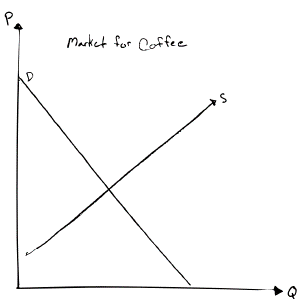
\includegraphics[width=.5\textwidth]{../figs/coffee1.png}
    \caption{Coffee market}
    \label{fig:coffee1}
\end{figure}

\subsection*{Part A}
Draw the total surplus at the market equilibrium, identifying consumer surplus and producer surplus.

\vspace{2mm}

\subsection*{Part B}
Now suppose the government imposes a tax on consumption of coffee.

\vspace{2mm}

\begin{enumerate}
    \item Illustrate the impact of the tax on the market equilibrium; what happens to P and Q?
    \item What happens to consumer surplus?
    \item Producer surplus?
    \item Total surplus?
\end{enumerate}

\vspace{2mm}

\subsection*{Part C}
Now suppose the government provides a subsidy to producers for each cup of coffee they sell, and answer the same questions as in Part B.

\vspace{2mm}

\subsection*{Part D}
With the two policies, does the government increase or decrease total surplus? How does the change in total surplus compare to the change in government revenue?

\vspace{2mm}

\section*{Question 3}
Let's consider the market for iPhones.

\subsection*{Part A}

Is the demand for iPhones elastic or inelastic? What about supply?

\vspace{2mm}

\subsection*{Part B}

Assume supply and demand are both fairly elastic (slope around 1). Illustrate the impact of a decrease in the cost of production, and show the change to surplus.

\vspace{2mm}

\subsection*{Part C}

Now suppose that the demand curve for iPhone is very inelastic (close to vertical), and answer the same questions.

\end{document}